%!TeX root=MemoriaTFG.tex
\chapter{Simulación de trayectorias} \label{chapter:Simulation}
Se define como simulación de una trayectoria al proceso por el cual, mediante los 
valores medibles y cuantificables extraídos del proceso de análisis, se recrea una 
trayectoria aleatoria que cumpla los mismos criterios. El proceso de simulación de esta 
propuesta tiene dos procesos principales. Primero (figura
\ref{figure:TrackGenerationSegments}) generar el camino dada las probabilidades 
analizadas desde el nodo inicio seleccionado. Posteriormente se realiza la simulación 
de la trayectoria por el camino seleccionado (figura \ref{figure:TrackGenerationPoints}).
En las siguientes secciones se describe estos dos procedimientos en detalle.
\begin{figure}[!htb]
\begin{minipage}{0.48\textwidth}
\centering
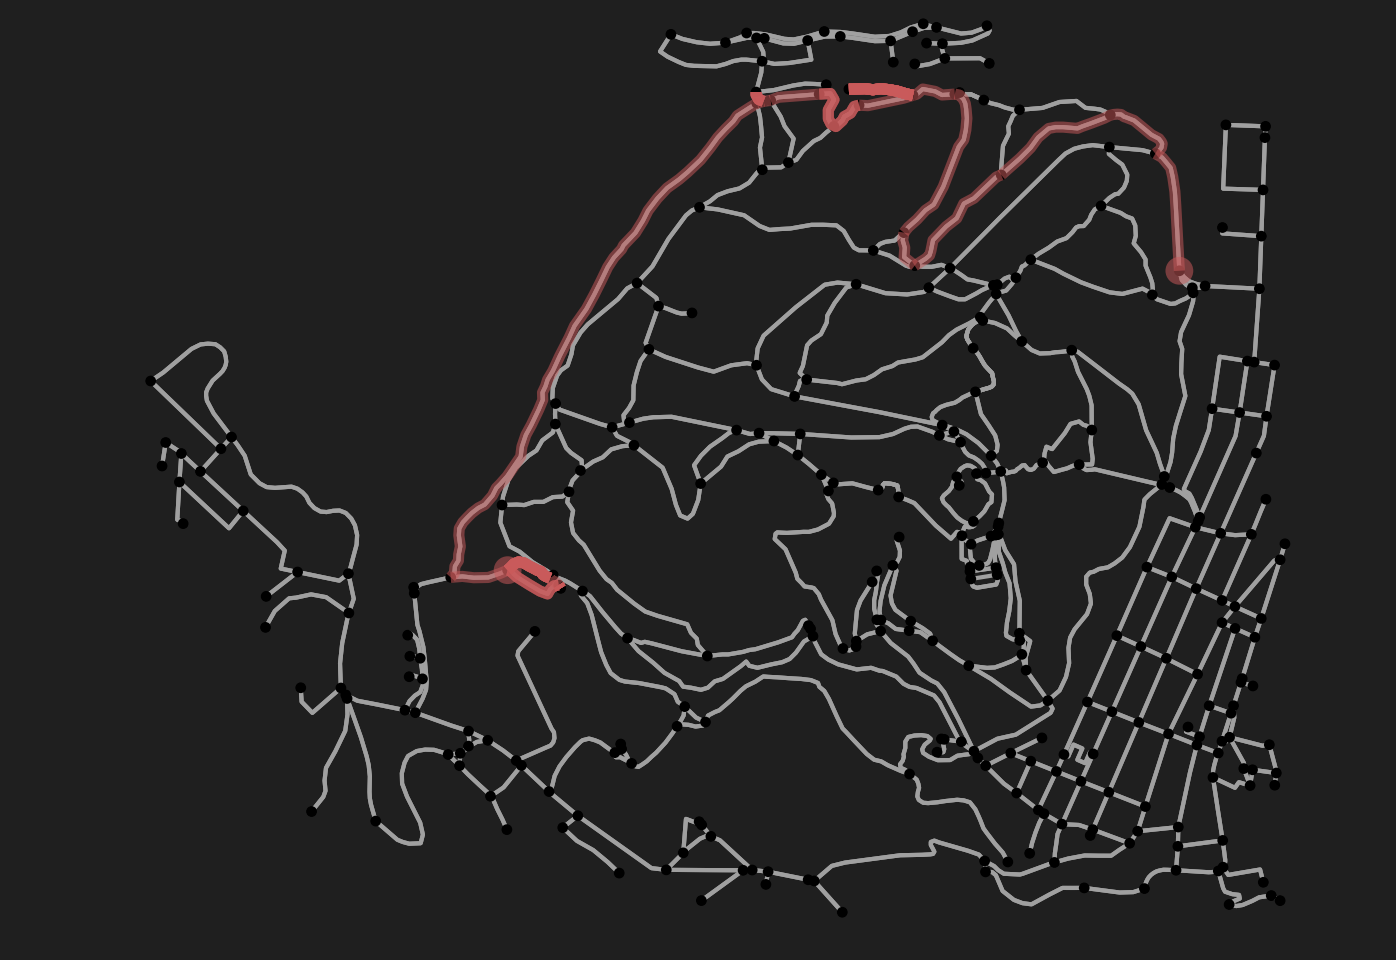
\includegraphics[width=1\textwidth]{./Imagenes/TrackGenerationSegments.png}
\caption{Generación de camino.}
\label{figure:TrackGenerationSegments}
\end{minipage}\hfill
\begin{minipage}{0.48\textwidth}
\centering
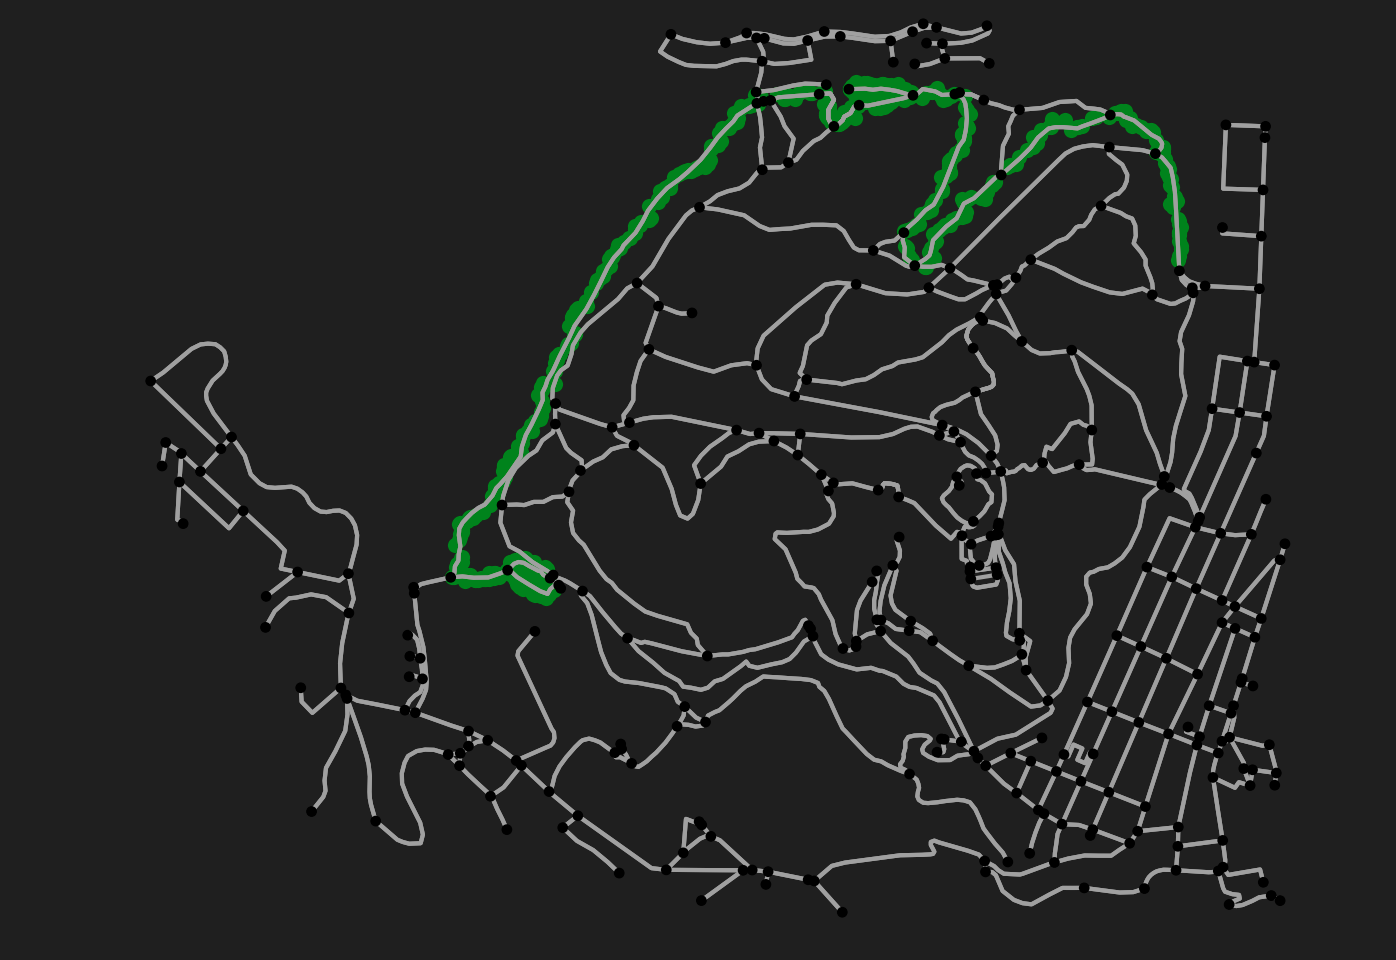
\includegraphics[width=1\textwidth]{./Imagenes/TrackGenerationPoints.png}
\caption{Generación de puntos.}
\label{figure:TrackGenerationPoints}
\end{minipage}
\end{figure}


\section{Generación de un camino}
La estructura lógica comentada en la sección \ref{section: EstructuraLogica} permite 
almacenar en las aristas la información referente a la frecuencia relativa de paso.
Para generar un camino se realiza un proceso iterativo por el cual, mediante un nodo 
origen asignado por parámetro de entrada, se selecciona uno de los caminos, 
manteniendo la distribución probabilística del conjunto de aristas, de forma que si una 
de las aristas tiene una frecuencia del 25\% de las detecciones, con un número 
suficiente de muestras se cumplirá dicha distribución. 
\begin{figure}[!htb]
\begin{center}
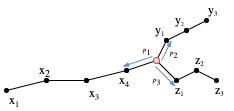
\includegraphics[width=0.75\textwidth]{./Imagenes/SimulationProbabilities}
\caption{Ejemplo de probabilidades dentro de un nodo intermedio entre rutas.}
\label{figure:PointGeneration02}
\end{center}
\end{figure}

El proceso de selección de aristas continúa hasta que la suma de las distancias 
acumule el total de distancia por recorrer, que será otro de los parámetros de entrada.
La implementación de este proceso se encuentra en el método \textit{create\_path} de 
la implementación del \textbf{\textit{interactor}} \textit{simulate\_track\_impl}.

\begin{lstlisting}[caption={Método create\_path}
\label{algoritmo:create_path},language=Python] 
    def create_path(self, origin, dist):
        path = []
        distance_created = 0
        prev_node = origin
        path.append(origin)
        while distance_created < dist:
            next_node = self.get_most_frequent_node(prev_node, path)
            distance_aux = distance_created + self.graph.get_edge_by_nodes(prev_node, 
            next_node)['length']
            if distance_aux < dist:
                distance_created = distance_aux
                path.append(next_node)
                prev_node = next_node
            else:
                return path, distance_created
        return path, distance_created
\end{lstlisting}

\section{Generación de los segmentos}
Una vez se tiene seleccionado el camino que se realizará se simula cada uno de los 
segmentos individualmente. Para ello se identifica el nodo origen y final del segmento y 
se generan todos los puntos necesarios hasta que la distancia a ese punto sea menor a 
una $d$, donde $d$ es una distancia parametrizada y modificable. La implementación 
de este proceso se encuentra en el método \textit{simulate\_segment} de la 
implementación del \textbf{\textit{interactor}} \textit{simulate\_track\_impl}.

\begin{lstlisting}[caption={Método simulate\_segment}
\label{algoritmo:simulateSegment},language=Python] 
    def simulate_segment(self, segment):
        aux = 0
        origin_node = segment[0]
        target_node = segment[1]
        segment = []
        origin_point = TrackPoint(self.graph.get_nodes()[origin_node]['x'], 	
        self.graph.get_nodes()[origin_node]['y'])
        target_point = TrackPoint(self.graph.get_nodes()[target_node]['x'], 
        self.graph.get_nodes()[target_node]['y'])
        try:
            dest, aux = self.calculate_point(segment, origin_node, target_node, origin_point, 
            target_point)
            next = dest
            while aux > DISTANCE_TO_FINAL_NODE:
                dest, aux = self.calculate_point(segment, origin_node, target_node, next, 
                target_point)
                next = dest
        except KeyError:
            pass
        return segment
\end{lstlisting}

\newpage
\section{Generación del punto pseudo-aleatorio}
Es en este punto de la propuesta donde se realiza la generación de puntos de forma 
\textit{pseudo-aleatoria}, utilizando información procedente de los análisis realizados. 
Para la creación de un punto a partir de otro se necesita una distancia $d$ y un ángulo 
$\alpha$ como se muestra en la figura \ref{figure:PointGeneration01}.
\begin{figure}[!htb]
\begin{center}
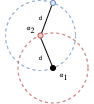
\includegraphics[scale=0.75, width=0.3\textwidth]{./Imagenes/PointGeneration01}
\caption{Ejemplo de generación de punto a partir de una distancia $d$ y un ángulo $
\alpha$.}
\label{figure:PointGeneration01}
\end{center}
\end{figure}

Cada punto será generado teniendo en cuenta el punto anterior. Se encuentra la 
proyección del segmento más cercano y se centra el ángulo de direccionamiento en el 
nodo inmediatamente posterior, con una desviación $\beta$ parametrizada y 
modificable. El proceso queda ilustrado en la figura \ref{figure:PointGeneration02}

\begin{figure}[!htb]
\begin{center}
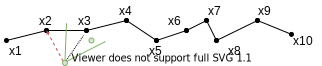
\includegraphics[width=0.75\textwidth]{./Imagenes/PointGeneration02}
\caption{Ejemplo de detección de proyección cercana y generación de punto.}
\label{figure:PointGeneration02}
\end{center}
\end{figure}

La distancia para la generación del punto se obtiene de una elección aleatoria siguiendo 
un proceso llamado \textit{Inverse transform sampling}, en el que se genera un número 
pseudo-aleatorio a partir de una función acumulativa dada una distribución 
probabilística \cite{Sigman01}.

La distribución probabilística de la distancia punto a punto se obtiene a partir de la 
información que se genera en el proceso de análisis. Se puede ver un ejemplo de esta 
información en la figura \ref{figure:PointToPoint} mostrada en la sección \ref{section: 
AnalisisDistancias}.

\section{Exportación de trayectoria a fichero \ac{GPX}}
En esta sección se describe la funcionalidad del aplicativo para realizar la exportación a 
\ac{GPX}. Esta funcionalidad es la que establece una salida al proceso de la aplicación 
y que permite que la trayectoria pueda ser almacenada, manipulada, visualizada y 
usada en otras aplicaciones.

Como salida del proceso  de simulación de una trayectoria se obtiene una lista de 
puntos. Esta lista es transformada en el formato válido a partir del \textit{resource} 
\textit{gpx\_resource}. Es la implementación de esta interfaz la que utiliza la librería 
\textit{gpxpy}. 

El método \textit{write} de la interfaz se encarga la creación de un directorio con el 
formato fecha y hora YYYYmmdd\_HHMM00 (Por ejemplo 20200503\_150300). La 
hora está configurada en formato \ac{UTC}. Posteriormente se genera una sola 
\textit{track} y segmento, y cada punto es convertido en un \textit{trackpoint} de este 
formato. Finalmente, se genera esta trayectoria y se crea un fichero con identificador 
único \ac{UUID} (simulated\_track\_d9cac860\-775d\-4454\- 
b8c4\-4b97f8530bfe.gpx) y se vuelca la representación \ac{XML}. Este proceso se 
implementa en método \textit{create\_gpx\_track} que vemos en el algoritmo 
\ref{algoritmo:create_gpx_track}.

\begin{lstlisting}[caption={Método create\_gpx\_track}
\label{algoritmo:create_gpx_track},language=Python] 
def create_gpx_track(data):
    gpx = gpxpy.gpx.GPX()
    gpx_track = gpxpy.gpx.GPXTrack()
    gpx.tracks.append(gpx_track)
    gpx_segment = gpxpy.gpx.GPXTrackSegment()
    gpx_track.segments.append(gpx_segment)
    [gpx_segment.points.append(gpxpy.gpx.GPXTrackPoint(point[1], point[0])) for point 
    in data]
    return gpx.to_xml()
\end{lstlisting}